\documentclass{muthesis2021}
\usepackage[numbers]{natbib}
\setcounter{secnumdepth}{4} % make subsubsection have numberings
\usepackage{graphicx}
\usepackage{latexsym}
\usepackage{amssymb,amsmath,amsthm,graphicx,mathrsfs}
\usepackage{url}
\usepackage{textcomp}
\usepackage{fontspec}

\usepackage{caption,setspace}
%\usepackage{caption}
\captionsetup{font={stretch=1.5}} % make the table,figure captions also have 1.5 linespacing

\usepackage[flushleft]{threeparttable}
%\usepackage{notoccite}
\graphicspath{ {../figures/} } % path to figures; you can put multiple of them. Just put them in separate brackets
\newcommand\mathplus{+}

\makeatletter
\renewcommand{\@dotsep}{10000} % set distance between dots to make it disappear in the table of contents
\setlength{\@fptop}{0pt}
\setlength{\@fpbot}{0pt plus 1fil}
\makeatother

% title of thesis -- nouns and stressed words should begin
\title{Improving Data Analysis of Incomplete Tabular Data by Graph Representation from Graph Neural Networks}

\author{Phaphontee Yamchote}


\candidate{Phaphontee Yamchote} % your name (without title)

\candidatetitle{Mr.\ } % Mr.\ Miss.\ or Ms.\ 

\degree{PhD} % default is MSc

\subject{Computer Science} % subject area of your thesis 

%\submissionyear{} % default is current year -- but maybe you will
                  % want to print it out again next year

%\isbn{974-04-xxxx-x} % remember to replace the x's when you know the number

% information for page i (advisors)

% NOTE: to avoid hyphenation in names on the abstract page, try
% putting the name which is hyphenated inside \mbox{ }
\majoradvisor{Thanapon Noraset} % name of supervisor (without title)
% default title is Lect.\
\majoradvisortitle{Dr. } % Dr.~ or Asst.~Prof.~ or Assoc.~Prof.~ or Prof.~  
\majoradvisorletters{Ph.D.} % Ph.D. or Dr.rer.nat.
\majoradvisorsubject{Computer Science} % subject in which advisor obtained last degree

\coadvisor{Chainarong Amornbunchornvej} % name of co-advisor
\coadvisortitle{Dr. } % title of co-advisor
\coadvisorletters{Ph.D.} % Ph.D. or Dr.rer.nat.
%\coadvisorstatus{Major advisor} % default is co-advisor but you might want
				% to classify him/her as a joint major advisor
\coadvisorsubject{Computer Science} % subject in which co-advisor obtained last degree

%\coadvisorII{Damon W. Ellison} % in case you have two co-advisors
%\coadvisorIItitle{MAJ }
%\coadvisorIIletters{Ph.D.}
%\coadvisorIIsubject{Molecular Microbiology and Microbial Pathogenesis}

%\coadvisorIII{} % in case you have three co-advisors
%\coadvisorIIItitle{}
%\coadvisorIIIletters{}
%\coadvisorIIsubject{}

\programchair{Asst. Prof. Boonsit Yimwadsana} % chair of your degree program
\programchairqual{Ph.D. (Electrical Engineering)} % qualifications of program chair
\faculty{Information and Communication Technology}
%\facultyI{Information and Communication} % Faculty name is not too long
%\facultyII{Technology} % Faculty name is too long to fit in one line

% default graduate studies dean is Prof.~M.R.~Jisnuson Svasti, Ph.D.
%\graduatestudiesdean{Prof. Patcharee Lertrit,\\M.D., Ph.D. (Biochemistry)}
\graduatestudiesdean{Prof. ........................}
%\GSDqual{Ph.D.} % this is no longer used
%\GSDstatus{Acting} % in case the dean is away and you need to put
		   % `Acting Dean' on the form 

% information for page ii (exam committee)

\submissiondate{January 5, 2021} % date of submission

\chair{...........................}
\chairqual{Ph.D. (Computer Science)} % qualifications of chair
%\memberI{Lect. Sudsanguan Ngamsuriyaroj} % use this if the major advisor is not present at the exam
%\memberIqual{Ph.D.} % qualifications of 1st member
%\memberIqual{Ph.D. (Computer Science and Engineering)} % qualifications of 1st member
%\memberII{Assoc. Prof. Damras Wongsawang} % use this if the co-advisor is not present at the exam
%\memberIIqual{Ph.D.} % qualifications of 2nd member
%\memberIIqual{Ph.D. (Information Engineering)} % qualifications of 2nd member
\memberIII{............} % 3rd member
%\memberIIIqual{Ph.D.} % qualifications of 3rd member
\memberIIIqual{Ph.D. (Computer Science)} % qualifications of 3rd member
%\memberIV{} % 4th member
%\memberIVqual{} % qualifications of 4th member

\facultydean{......................}    % default is Prof.~Prasert Sobhon
\FDqual{Ph.D. (Computer Science)}         % default is Ph.D.
%\FDstatus{Acting} % in case the dean is away and you need to put
		   % `Acting Dean' on the form 

% information for page iv (ABSTRACT)

\candidatenumber{ 6436198 ITCS/D}
%\major{} % major of thesis (not necessary if the same as subject)
\keywords{MACHINE LEARNING / GRAPH NEURAL NETWORK} % 1st line of keywords
%\keywordsII{BIOINFORMATICS} % 2nd line of keywords
%\keywordsIII{ /  / } % 3rd line of keywords

% information for page v (THAI ABSTRACT)

%\thaisubject{{\Th วิทยาการคอมพิวเตอร์}} % thai name of degree subject
%\thaititle{{\Th การแนะนำเครื่องมือทางชีวสารสนเทศโดยอิงหลักฐานทางการใช้งาน}} % title of thesis in thai
%\thaicandidate{{\Th นางสาวอังคณา หวัง}} % your name in thai
%\thaimajoradvisor{{\Th อาจารย์อภิรักษ์ หุ่นหล่อ}} % Thai name of advisor (if they are Thai)
%\thaicoadvisor{} % Thai name of co-advisor (if they are Thai)
% you might need to put the individual (first and last) names
% inside \mbox{} to stop them being split by the word-breaking routine

%\thaicoadvisorII{} % Thai name of 2nd co-advisor (if they are Thai)

% information for Biography

\dateofbirth{26 August 1992} % your date of birth
\placeofbirth{Bangkok, Thailand} % province and country of birth
\firstdegreeinstitution{Chulalongkorn University} % where you did your first degree
\firstdegreeyears{2012--2016} % years for 1st degree
\firstdegree{Bachelor of Science} % default is Bachelor of Science
\firstdegreemajor{Mathematics} % first degree major
%\longfirstdegree % necessary if you want the subject on the next line
\preinstitution{Chulalongkorn University, 2017--2021} % details of place you went before present degree if
		  % it wasn't your 1st degree
\preinstitutionLnII{Master of Science (Mathematics)} % 2nd line of details
%\preinstitutionII{} % details of 2nd place you went before present degree
%\preinstitutionIILnII{} % 2nd line of details
\years{2021--20..} % years taken to do your present degree
%\postinstitution{Mahidol University} % details of place where you continued your study for your
		   % present degree
%\postinstitutionLnII{} % second line of details
%\scholarship{} % details of 1st scholarship
%\scholarshipLnII{} % 2nd line of details (if necessary)
%\scholarshipLnIII{} % 3rd line of details (if necessary)
%\scholarshipII{} % 2nd scholarship
%\scholarshipIILnII{}
%\scholarshipIILnIII{}
%\scholarshipIII{}  % 3rd scholarship
%\scholarshipIIILnII{}
%\scholarshipIIILnIII{}
%\scholarshipIV{}  % 4th scholarship
%\scholarshipIVLnII{}
%\scholarshipIVLnIII{}
%\position{Data Analyst} % present position
%\workplace{Department of Virology, USAMD-AFRIMS} % location 
%\workplaceLnII{315/6 Rajvithi Road, Bangkok, Thailand} % second line of location
%\homeaddress{} % your home address if you do not have a position
%\homeaddressLnII{}
%\homeaddressLnIII{}
\email{yamchote\_p@outlook.com} % the email address at which you can be contacted after you have left


   

\def\Draft{true}
\newcommand{\paragraphHead}[1]{
	\ifthenelse{\equal{\Draft}{true}}{\paragraph*{[#1]}~\\}{~}
}  

\newcommand{\R}{\mathbb{R}}
\newcommand{\N}{\mathbb{N}}
\newcommand{\Z}{\mathbb{Z}}
\newcommand{\Q}{\mathbb{Q}}

\newtheorem{prop}{Proposition}[chapter]
\newtheorem{lem}[prop]{Lemma}
\newtheorem{cor}[prop]{Corollary}
\newtheorem{thm}[prop]{Theorem}
\newtheorem{fact}[prop]{Fact}



\theoremstyle{definition}
\newtheorem{defi}[prop]{Definition}
\newtheorem*{question}{Question}
\newtheorem*{rem}{Remark}
\newtheorem*{ex}{Example}
\newtheorem*{assumption}{Assumption}


\begin{document}

\maketitle

\linespacing{1.5}
\acknowledgements{First}

\abstract{%
\linespacing{1.2} % change the linespacing to fit the abstract in the allotted space
Your abstract goes here.
}
{
\linespacing{1.2} % change the linespacing to fit the abstract in the allotted space
Your thesis implication goes here.
} % point to english abstract.tex
% \thaiabstract{ภาษาไทย} % the Thai abstract doesn't work. Have to manually do it in Word. But leave this here so that the page number runs correctly.

\tableofcontents
\listoftables
\listoffigures
%\abbrlist
%\symlist

% your thesis goes here!
%

 % you can also have one input per chapter
\chapter{Introduction} \label{chap:intro}

\section{Motivation}
%\paragraphHead{about data}
%Nowadays, data plays an important role in both academia and business. They can find some
%business opportunities from their data. Then, the field of study that unifies engineering, mathematics, statistics, and computer science emerges, called data science. Data science is broadly
%used in business and industry to find the business opportunity hidden in data. Chatterjee et al. (2021) \cite{...} concluded that using data science in an enterprise increases accuracy in innovative
%decisions and the potentiality of competition in business.
%
%\paragraphHead{Tabular data: a format of data often used and also meet missing (merge to the first paragraph)}
%Tabular data is a format of data that displays in rows and columns.
%One of them corresponds to the collected features of each data sample.
%It is a ubiquitous data format used in practical applications in many domains such as enterprise operations, manufacturing, clinics, and surveys.
%For example, doctors or medical technologists may want to predict the chance of a specific disease for a patient from the patient’s historical records that are stored in the form of a table.
%Missing data problem is also a challenge in modeling tabular data.
%Even though tabular data has its own structure represented by feature vector, missing values can eliminates the structure of tabular data so that model cannot learn or compute on such data.
%%However, one of the efficient approaches that might fill this gap is to represent tabular data by graphs and to use graph neural networks (GNNs).

\paragraphHead{Data Science and Tabular data}
In the contemporary landscape, data holds significant value in academia and business by data-driven paradigm.
It drives the emergence of data science—an interdisciplinary field combining engineering, mathematics, statistics, and computer science.
Applications of data science span various industries, uncovering concealed business opportunities.
Research by Chatterjee et al. (2021) emphasizes its role in enhancing decision accuracy and fostering competitiveness.
Among many kinds of data's format, tabular data is one of the formats that is widespread in domains like healthcare and manufacturing.
It presents a structured means to store information.

\paragraphHead{tell that missing data is a problem often met}
However, not only mining or modeling data but also data preparation is a task that practitioners in data science have to do.
They spend much time in cleaning and organizing data.
One of the common challenges is missing features which is the problem of absence for some values in the given datasets.
This problem is relatively common in almost all research and all formats of data, especially in tabular data.
It can significantly affect results obtained from the data \cite{...} in sense of learning.


\paragraphHead{causes of missing data}
There are many causes of missing data.
First, the problem of measuring instruments is a cause that often occurs in a production line.
Second, some missing data can emerge from the nature of data,
such as different factors corrected between males and females in a clinical survey
or the disappearance of a patient during the treatment process.
Third, the lack of knowledge of the sample can also result in missing data.
There may be the case of the sample giving a ``don't know'' answer to an observer in some complicated question.
Even independence of each measurement process (i.e. each feature) can be considered as a cause of missing data in sense of feature.
That is, some feature can be determined by logical combination of two or more features.
However, independent measurement make such information hidden.

\paragraphHead{significance of missing data}
The missingness problem holds significant importance in machine learning and deep learning, primarily due to its computational implications.
In these fields, including the cutting-edge domain of deep learning, algorithms often rely on fixed-size representation vectors, also known as embeddings.
However, when dealing with missing data without proper preprocessing, a critical challenge arises as data cannot be directly fed into models due to the absence of vital information.
From a theoretical perspective, machine learning involves the search for an optimal distribution within a hypothesis class, guided by a given training dataset.
This search is essentially a quest to find the best model within an equivalent class of models.
However, the presence of missing data complicates this task by weakening the inductive bias of learning; so misleading the learning of models that much more models are equivalent to the model which should be.
In other words, the higher proportion of missing data, the more models in the same equivalence class.
This makes the learning algorithm more difficult to identify and learn the optimal models when working with datasets containing missing values.

%\paragraphHead{Imputation: the most basic solution}
%One of the simple way is to basically impute these missing values by a constant value, mean or interpolation.
%However, these imputation may not reflect the actual dataset.
%Actually, we do not even know the actual dataset.
%In addition, some missing behavior is also informative such as unrating the product from a customer which may mean dissatisfaction but the customer avoids giving a reason directly.
%So imputation seems that we do not concern the hidden information about missing data.
%Moreover, Ma, et al. (2018) \cite{Ma} commented that the imputation method ignores uncertainties of data which means as the same as hidden information said earlier.
%
%\paragraphHead{More a bit Imputation but with learning from data}
%Not only basic imputation methods, but many work also investigated imputation based methods by learning from data.
%However, it still relies on the assumption that all missing values can be replaced as a number.
%But not all missing scenario can be imputed, for example, unrating the product.
%Also the case of some non measurable feature depending on others, the value 0 and a missing value are not equivalent.
%Moreover, these methods is independent from the learning process.
%In other words, the same model may be lead to different way by different imputation methods.
%The only way is to cross test all possible imputation methods to see whether which method is the best one for the desired model.
%This still requires much effort and time-consumption in the process of feature engineering.
%
%\paragraphHead{Imputation: the most basic solution}
%A variety of methods exist for handling missing values, including straightforward approaches like replacing them with constants, means, or using interpolation.
%However, these methods may not accurately represent the true nature of the dataset.
%The challenge arises because the actual dataset is often unknown, and some missing patterns carry valuable information, such as a customer choosing not to rate a product, indicating potential dissatisfaction without specifying the reason.
%Imputation methods, in this context, may overlook the hidden information within missing data.
%Additionally, studies like Ma et al. (2018) \cite{Ma} argue that imputation methods disregard data uncertainties, echoing the earlier notion of hidden information.
%While more advanced imputation methods based on data learning have been explored, they still assume that all missing values can be numerically replaced, which is not always feasible—consider scenarios like product unrated or non-measurable features dependent on others.
%Furthermore, these methods operate independently of the learning process, meaning that the same model may yield different results based on the chosen imputation method.
%Consequently, determining the most suitable imputation method for a specific model often involves extensive cross-testing, demanding considerable effort and time in the feature engineering phase.

\paragraphHead{Brief Literature: existing methods which}
The most basic methods to handle this issue is imputation for the missing values.
Many work also attempts to find methods to impute missing data in various way including distribution-based imputation and learning the missing values as well.

******To the best of our knowledge, there is no state-of-the-art imputation methods.
Even in practice, the casewise deletion, i.e. removing the data points containing missing values, seems to be the most practical method if much more data is available. 

However, Ma et al. (2018) \cite{Ma} argue that imputation methods disregard data uncertainties, echoing the earlier notion of hidden information.
Even in some real-world case, missing values are their native structure which does not make sense to impute with value.





\paragraphHead{Brief Literature: GNN potential}
From the review of literature, we found an interesting framework addressing this issue in different perspective by graph, called GRAPE \cite{GRAPE}.
They proposed a framework that can learn from data containing missing values without imputation for these missing subjects.
GRAPE is a graph-based framework that table of data is represented by a graph which will be processed by an deep-network algorithm call graph neural networks (GNNs).
This demonstrates the potential that representing data by graphs and using GNN algorithms can weaken the need of completeness of datasets.
In other words, GNNs with graph data structure are more flexible in computation rather than using the fixed length of feature vector fed into algorithm directly.

Not only missing data, but GNNs are also used in many works that investigated approaches for modeling complete tabular data. 
There are both an idea of using one graph for the whole table \cite{grape} does and idea of using a dataset of graphs which of each corresponds to each instance of table \cite{...}.
It is a naive idea to use a big graph for the entire table to learn an hidden information inferred between row (instance) or column (feature).
On the other hand, some work uses a graph of instance to capture hidden information inside the instance among its feature value.


\paragraphHead{Brief Literature: Gap between GNN and missing data}
GRAPE is an sample algorithm that allows avoidance of imputation.
It is designed to capture the cooperating information between a node of instance and a node of feature that is observed for the instance and the captured information is aggregated to the node of instance to infer its corresponding label.
Technically, it seems to utilize the flexibility of GNNs to omit the missing feature by not using the information from that feature node.
However, some missing values may be informative in sense of structure.
They should be utilized in prediction, not abandoned.

In contrast, the another idea to represent tabular data by graph, which represents each instance by a graph, is still not explored to address missing issue.
So this motivates us to study how to address the missing data issue by the idea of graphs of samples because we believe that the graph of a sample should be effectively used for capturing dependency of missingness.

To the best of our knowledge, no work address the missing data by this idea.
However, tabular data is not native graph data structure.
So it comes up with the question of how to represent data by graphs and how to design GNN algorithm to process them.

\paragraphHead{How we will fill the gap}
To fill the aforementioned gap, this work proposes the end-to-end GNN framework from tabular data to predicted label.
The framework consists of two major modules: (1) graph construction and (2) prediction from graphs as shown in Figure \ref{framework}.

\begin{figure}[h]
	\centering
	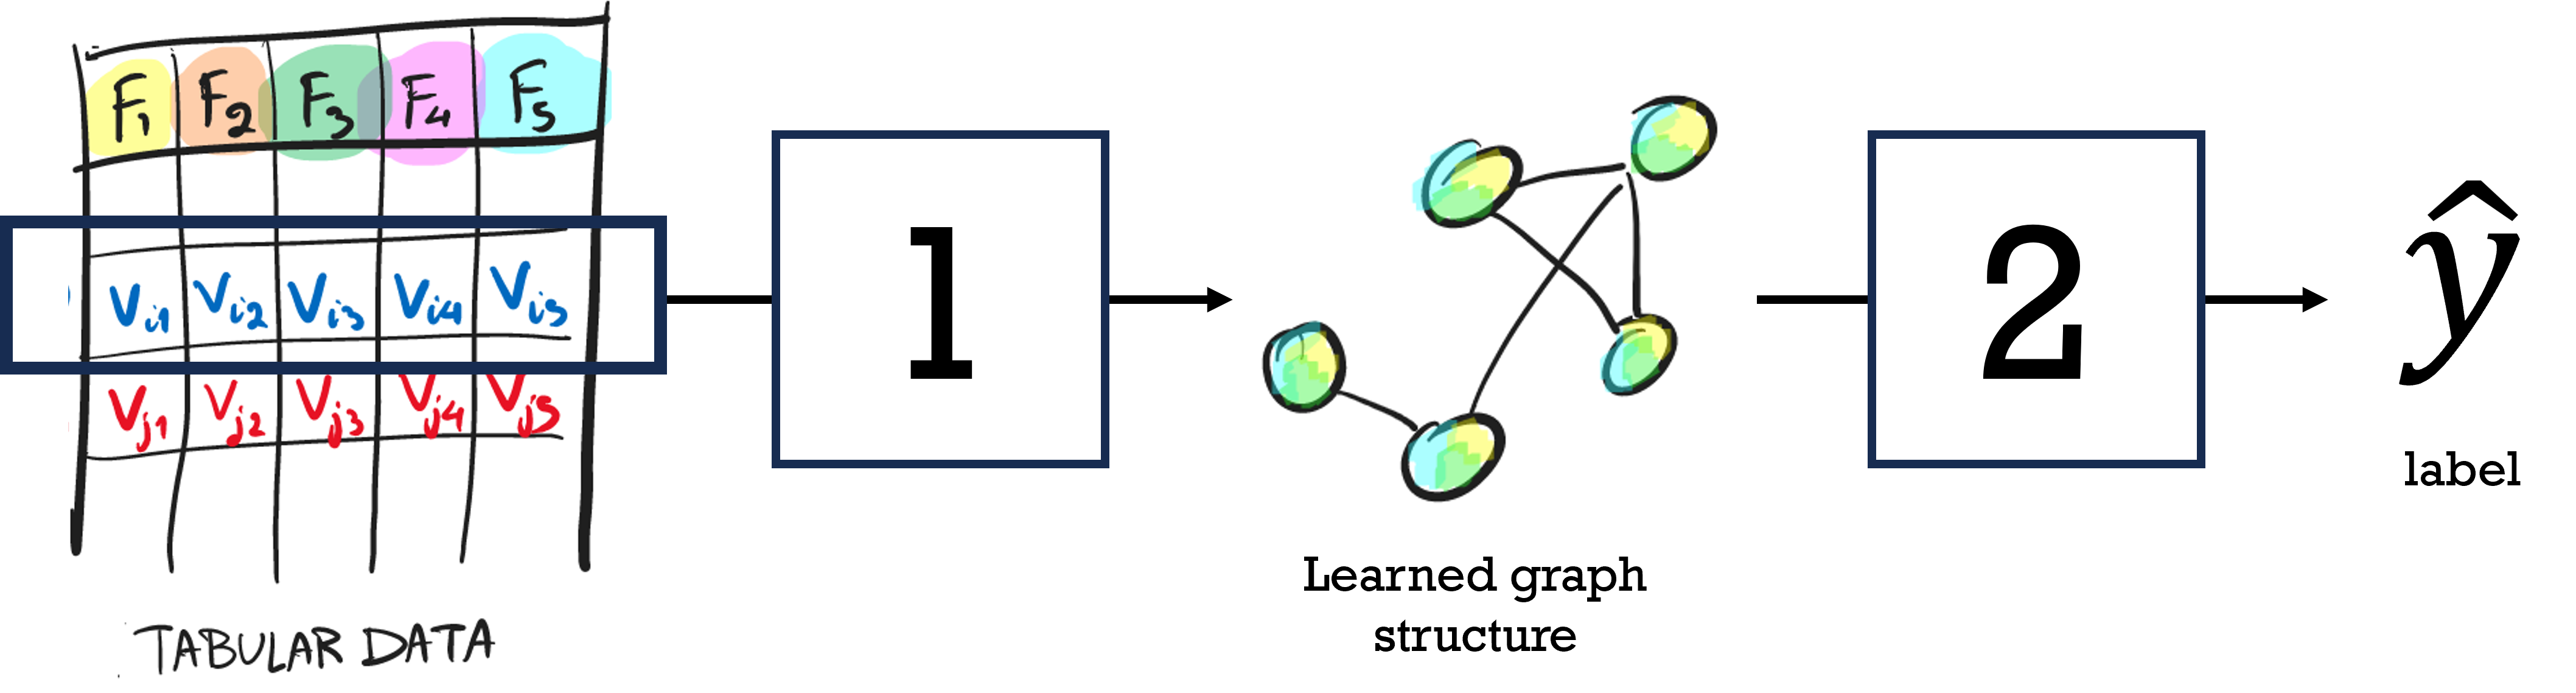
\includegraphics[width=0.7\linewidth]{framework}
	\caption{text}\label{framework}
\end{figure}

% [] want to include idea that complete graph may introduce much noise not related
 
The graph construction module is for learning the structure of a graph of a given data point which is used as a graph representation of the instance.
Since some missing values is caused by dependency of values of other features, e.g. not measurable attribute in male patient, we aim to develop a graph structure learning module so that it can keep dependency between features.
Not only dependency, interaction between feature, i.e. the higher-order nonlinear operation between features is also an interesting characteristic of tabular data that can be considered as a missing value.
Hence we also aim that this module of our work can also keep the interaction information in the learned graph structure.

On the other hand, we then develop the module making prediction from the learned graphs.
This prediction is aimed to be robust for missing values, noise features, dependency and also interaction.


%\paragraphHead{It's time to tell about graphs and GNNs: graph first}
%From the issue of missing data, we need a learning algorithm or a data structure that is more flexible in computation rather than using the fixed length of feature vector fed into algorithm directly.
%This work concentrates on graphs data structures and graph neural network (GNN) algorithms.
%As we have ever seen in data structure, graphs are flexible in how to storage data via edges and nodes.
%Moreover, they are suitable to be flexibly computed by using edges. 
%
%\paragraphHead{It's time to tell about graphs and GNNs: GNNs next}
%GNNs are a class of neural based methods designed to perform inference on graph data.
%It has emerged as a promising approach for modeling structured and semi-structured data, such as social networks \cite{Zhang2019}, molecular structures \cite{Gilmer2017}, and knowledge graphs \cite{Schlichtkrull}.
%Particularly when dealing with high-dimensional or incomplete datasets, GNNs have demonstrated superior performance in various applications, as they effectively capture complex dependencies among nodes and edges in a graph \cite[Kipf \& Welling 2017]{GCN}.
%Moreover, GNNs have advantages over traditional machine learning methods as they do not rely on assumptions about independence of instances and features.
%This makes GNNs are more flexible in learning with respect to both data they use and computation they do.

%\paragraphHead{Conclude to our expectation to use graphs and GNNs to address missing data problem}
%Therefore, the objective of this work is to investigate the new method to learn representations or embeddings of tabular data containing missing values by using GNNs.
%We also aim to find a new way to represent tabular data by a graph.
%The proposed algorithm will allow users to directly feed a data point from tabular data containing missing values without any preprocessing process.
%Moreover, the model can be trained in an end-to-end fashion.

\section{Research Objectives}
%\subsection*{Problem Statement}
%Missing data, which often occurs in many domains of tabular data, can lead to biased or inaccurate models if not handled properly.
%Current methods for handling missing data, such as imputation, can introduce additional assumptions and may not capture the underlying structure of the data.
%Moreover, doing so in the process of feature engineering takes much time and effort of practitioners.
%We seek to develop an approach that can effectively handle missing data in datasets without relying on process of data preparation for missing values such as imputation.
%Our model is also aimed to be able to learn the information of missing values in the sense of natural missing value

%\subsection*{Research Questions}

%\subsection*{Objectives}
The primary objective of this research is to investigate a GNN-based framework that can address the challenge of missing data. The further detail of our objectives is as follows:

\begin{enumerate}
	\item develop an algorithm to construct spare graph structures for the representation of data that can be efficiently used for computation of the corresponding GNN prediction algorithm and maintain the interaction inside the data instance,
	\item develop a GNN algorithm that can be trained by datasets containing missing values without any preprocessing, and also can predict the corresponding label of the given data that may contain missing values.
	\item Validate the developed model both synthetic and real-world datasets.
\end{enumerate}

\section{Outlines}
In Chapter \ref{chap:litrev}, we explain more detail related to our work including graph representation, GNNs and related work.
Readers can find deep detail and also formal definition in the section preliminary of this chapter.
And then, we describe how we perform this research in Chapter \ref{chap:meth}: methodology.


\chapter{Literature Review} \label{chap:litrev}
%\begin{center}
%	============ [below is old] ===============
%\end{center}

\section{Related Work}
%\subsection{Handling Missing Data}(move to prelim if needed)
%Many works investigated methods to deal with this problem.
%In addition to statistical imputation, some work developed new methods in machine learning approaches to impute missing data.
%For example, Samad and Harp dealt with missing values by self-organizing map (SOM) \cite{SOM}.
%Many works use multi-layer perceptron (MLP), for example, \cite{MLP,MLP3,MLP2}.
%Moreover, there are also works using deep learning approaches, for example, \cite{GAIN, GRAPE}.
%However, there also are works dealing with this problem by avoiding imputation.
%They try to learn a representation of data instead of imputation.
%These works are based on the hypothesis that missingness should be informative, and imputation is the method that ignores uncertainties in missing data.
%
%content...

\subsection{Graph Neural Networks for Tabular Data}
GNNs have been applied to diverse types of tabular data, including healthcare \cite{Mao2019} and financial data  \cite{Seo2018}. Their ability to model complex interactions and dependencies between variables \cite{Zhang2018, Monti2018} and handle missing values \cite{GRAPE} make them advantageous for tabular data analysis. However, designing GNNs for tabular data requires careful consideration of factors such as graph structure and feature engineering \cite{Hu2019}. The graph structure should reflect the relationships between variables, while feature engineering should effectively transform input features into graph structures suitable for GNN models.

content...

\subsection{Graph Neural Networks for Missing Data}
content...

%\begin{enumerate}[label=(\Roman*)]
%	\item What is missing issue
%	\item Why is it significant
%	\item way to handle
%\end{enumerate}

\section*{*****************************log*****************************}


%As aforementioned, we can categorize the methods of handling missing data into two groups.
%The first group is imputation before using, and the second group is learning representation of
%data by deep learning. We argue that excluding ease of usage and low resource consumption
%imputation is inappropriate because it is impossible to fill the correct values. Therefore, learning
%the representation of data is a fascinating method. Moreover, this method is successful in many
%domains of machine learning.



Missing data is significant because it can lead to biased model performance and inaccurate predictions. Handling missing data can be done through various methods such as statistical imputation, machine learning-based imputation, and deep learning-based imputation. Statistical methods such as mean imputation, regression imputation, and hot-deck imputation assume that the missing values follow a certain statistical distribution, but they might not be accurate if the missing values are not random. Machine learning methods like k-nearest neighbor (KNN) imputation \cite{missingDNA} and decision tree-based imputation \cite{missingTree} can be effective when the missing values have some patterns, but they might not work well if the missingness is too extensive. Deep learning methods such as autoencoders \cite{missingAutoen} and Generative Adversarial Networks (GANs) \cite{GAIN} can be used to impute missing values, but they require a large amount of training data and computational resources, and their performance might not be better than simpler imputation methods \cite{Garcia}.

However, A limitation of imputation methods is that they assume that the missing values can be imputed based on the observed values and other relevant variables. However, in practice, we may not know the exact values of the missing data, and imputing them may introduce errors and bias in the analysis. Moreover, in some cases, the missing data itself may be informative, and imputing them may lead to loss of information. Therefore, it is important to carefully consider the nature of missing data and the suitability of different imputation methods before making any assumptions or decisions.

Recent research has shown that deep learning techniques can also be applied to handle missing data. One such approach is GAIN \cite{GAIN}, proposed by J. Yoon et al. in 2018, which utilizes Generative Adversarial Nets (GANs) to generate plausible values for missing data based on the observed data. Another study by M. Smieja et al. \cite{Smieja} in 2019 also explored the use of neural networks for processing missing data, where a deep network was used to predict data containing missing values based on the observed values without imputation. In 2020, Ghorbani et al. \cite{Ghorbani} proposed a novel method called Embedding for Informative Missingness (EFIM), which uses a deep learning model to learn embeddings of the missing values that preserve their informativeness. The embeddings are then used to predict the corresponding label of input via the model that is learned together with the embedding. These recent studies suggest that deep learning-based methods can be effective for handling missing data, but they still ignore the dependencies of features on missing values.

In this work, we aim to develop a framework for handling missing data that does not rely on explicit imputation. Specifically, we want to design a model that can predict the label of a given data point even if some of its features are missing, without necessarily imputing the missing values. If necessary, the model should also be able to reconstruct the missing parts of the input based on the other nonmissing features. Our proposed approach will leverage deep learning techniques to capture the complex relationships between the input features and the label, as well as the dependencies between the missing and nonmissing features. By doing so, we hope to provide a more accurate and robust solution to the missing data problem, while also preserving the integrity of the original data.




%\section{Deep Learning for Tabular Data}
%\begin{enumerate}[label=(\Roman*)]
%	\item Challenges of deep learning for tabular data:
%%	\begin{enumerate}[label=\arabic*.]
	%%		\item Missing data
	%%		\item Feature interaction
	%%		\item Feature selection
	%%	\end{enumerate}
%
%			Deep learning models have shown amazingly success in many fields such as image and text, but they still underperform compared to tree-based models in tabular data analysis. \cite{Grinsztajn}
%			One of the major challenges in deep learning for tabular data is the presence of missing data, as many real-world datasets often have incomplete data, which can affect model performance.
%			Feature interaction is another challenge, as deep learning models struggle to capture complex interactions between features, which can lead to poor model performance.
%			Finally, feature selection is an important consideration, as deep learning models tend to perform poorly with a large number of features, and selecting the most relevant features can significantly improve model performance.
%			Not only what I have mentioned, but also high-dimension, heterogeneity, imbalanced data and limitation of interpretability are challenges for deep learning of tabular data.
%	\item Recent advances in deep learning for tabular data:
%	
%			Recent advances in deep learning for tabular data have shown promising results in various real-world applications. One approach is to use neural networks with architectures specifically designed for tabular data such as the TabNet and AutoInt models (Su et al., 2020; Liang et al., 2020).
%			Another approach is to incorporate graph neural networks (GNNs) to capture feature interactions and handle missing data, such as the work by Chen et al. (2021) and Huang et al. (2021).
%			However, these methods still face challenges such as the curse of dimensionality and the need for effective feature selection and preprocessing techniques (Guo et al., 2021; Yuan et al., 2021).
%			Overall, the recent advances in deep learning for tabular data show great potential, but further research is needed to address the challenges and improve the performance of these models in real-world scenarios.
%			
%	\item Comparison of deep learning and traditional machine learning for tabular data in performance:
%	
%			Numerous studies have compared the performance of deep learning and traditional machine learning methods for tabular data. Some studies found that deep learning models outperform traditional machine learning models on certain datasets, such as those with high-dimensional and complex features, while others found that traditional machine learning models perform better on datasets with small to medium-sized features. For example, Wang et al. (2019) found that deep learning models outperformed traditional machine learning models on a dataset with high-dimensional features. In contrast, other studies, such as Wang et al. (2018) and Johnson et al. (2019), found that traditional machine learning models, such as random forests and gradient boosting machines, outperformed deep learning models on certain tabular datasets. Despite these mixed results, it is clear that both deep learning and traditional machine learning methods have their strengths and weaknesses when it comes to tabular data analysis, and the choice of method should depend on the specific characteristics of the dataset and the research question at hand.
%\end{enumerate}
According to Grinsztajn (2022) \cite{Grinsztajn}, deep learning models have generally not performed as well as traditional machine learning models, particularly tree-based models, in tabular data analysis.
As discussed in the previous section, there are several challenges that contribute to this underperformance.
Recent advances in deep learning for tabular data have incorporated neural networks with architectures specifically designed for tabular data, TabNet \cite{Tabnet} for example.
Some work attempts to capture feature interactions \cite{Table2Graph} which is simply an operation among two or more features with respect to the output variable such as multiplication between two features, and handle missing data \cite{GRAPE}. 
However, these methods can be computationally expensive.
Table2Graph, for instance, uses a reinforcement learning approach that requires significant amounts of data and computation power to address feature interactions. GRAPE, on the other hand, models a table of data as a graph to handle missing data but does not address feature interactions.

Numerous studies have compared the performance of deep learning and traditional machine learning methods for tabular data. Some studies found that deep learning models outperform traditional machine learning models on certain datasets, such as those with high-dimensional and complex features, while others found that traditional machine learning models perform better on datasets with small to medium-sized features. For example, Ching et al. (2018) \cite{Ching2018} found that deep learning models outperformed traditional machine learning models on a dataset with high-dimensional features.
In contrast, other studies, such as Grinsztajn et al. (2022) \cite{Grinsztajn}, Olson et al. (2018) \cite{Olson2018}, and Fernández et al. (2014) \cite{Fernández} found that traditional machine learning models, such as random forests and gradient boosting machines, outperformed deep learning models on certain tabular datasets. Despite these mixed results, it is clear that both deep learning and traditional machine learning methods have their strengths and weaknesses when it comes to tabular data analysis, and the choice of method should depend on the specific characteristics of the dataset and the research question at hand.


%\subsection{Graph Neural Network}
%
%\section{Related Work}
%\subsection{Graph Neural Networks in Tabular Data Analysis}
%\begin{enumerate}[label=(\Roman*)]
%	\item Previous research on using GNNs in tabular data analysis
%	\item Advantages of using GNNs in tabular data analysis
%	\item Design considerations for GNNs in tabular data analysis
%\end{enumerate}
%	Before delving into the potential of Graph Neural Networks (GNNs) in modeling tabular data, it is important to understand the limitations of traditional machine learning models. Tabular data often consists of structured and semi-structured data with complex dependencies among the features. This complexity can be difficult to capture with traditional models, especially when the data is high-dimensional or has missing values. While deep learning models have shown great success in modeling complex data such as images and text, they have struggled to achieve similar results with tabular data due to the lack of inherent structure and the difficulty of learning meaningful representations. In recent years, however, GNNs have emerged as a promising approach for modeling structured and semi-structured data, such as social networks, molecular structures, and knowledge graphs. GNNs have been shown to be effective in capturing complex dependencies among nodes and edges, and have demonstrated superior performance compared to traditional methods in various applications. Therefore, exploring the potential of GNNs in modeling tabular data could pave the way for more accurate and interpretable models, as well as new insights into the relationships between features in the data.
%	
%	GNNs are a class of neural networks that can learn representations of nodes and edges in a graph, even representations of graphs, which allows them to capture the structural information of the graph in the forms of message passing.
%	One of the key advantages of GNNs is their ability to learn the relations between nodes in a graph, which enables them to model complex interactions between the nodes (Kipf \& Welling, 2017) \cite{...}.
%	This is particularly useful in many real-world applications such as social network analysis, recommendation systems, and drug discovery.
%	Moreover, GNNs have shown superior performance compared to traditional machine learning models and deep learning models in many graph-related tasks.
%	They can handle large-scale graphs efficiently and provide a better representation of the graph structure, which allows them to achieve better results in many graph-related tasks such as node classification, link prediction, and graph classification (Wu et al., 2020) \cite{...}.
%	Moreover, the assumptions on which GNNs rely are weaker than what traditional machine learning and deep learning need, such as independence of data points \cite{...}.
%	The advantages of GNNs make them a promising area of research in the field of machine learning and graph analysis.
%
%	Besides the tasks whose data is explicitly in the forms of graphs, such as networks or molecules, recent studies have explored the potential of using Graph Neural Networks (GNNs) in tabular data analysis.
%	GNNs have been applied to various types of tabular data, such as healthcare data (Choi et al., 2020; Shang et al., 2019) \cite{...} and financial data (Wang et al., 2021) \cite{...}.
%	These studies have demonstrated the effectiveness of GNNs in capturing complex relational information in tabular data that cannot be easily captured by traditional machine learning models.
%	One of the main advantages of using GNNs in tabular data analysis is that they can capture complex interactions and dependencies between different variables in the dataset.
%	Moreover, GNNs can handle missing values, which is a common challenge in tabular data analysis (Wu et al., 2021).
%	However, designing GNNs for tabular data analysis requires careful consideration of several factors, such as the choice of graph structure and feature engineering (Yin et al., 2020).
%	For instance, the graph structure should reflect the relationships between variables in the dataset and feature engineering should ensure that the input features can be effectively transformed into graph structures that can be processed by the GNN model.
%	Overall, the research on using GNNs in tabular data analysis suggests that GNNs hold promise as a powerful tool for handling complex tabular data and would  be explored further in this research.



%\subsection{Missing Data Handling with GNNs}
%\begin{enumerate}[label=(\Roman*)]
%	\item 
%	\item 
%	\item 
%\end{enumerate}

%	Graph representation learning has recently emerged as a promising approach for handling missing data, which is the main goal of this work.
%	One notable work in this area is GRAPE, proposed by You et al. in 2020 \cite{...}.
%	GRAPE is a framework utilizing GNNs for feature imputation and label prediction with missing data.
%	It constructs a bipartite graph from the data matrix, where samples and features are two types of nodes and observed values corresponding to each sample and each feature are attributed edges.
%	It then formulates the feature imputation as an edge-level prediction task and the label prediction as a node-level prediction task.
%	
%	Danel et al. (2020) \cite{...} also proposed another related work handling missing issue, but in image, to process incomplete images as graphs, where each node is a visible pixel and each edge connects neighboring pixels.
%	The graphs are then fed to a spatial graph convolutional neural network (SGCN), which can mimic image convolutions and handle missing data without imputation.
%	However, it only considers spatial graph convolutions, which are based on the Euclidean distance between nodes. There may be other types of graph convolutions that can capture more complex relationships between pixels, such as spectral graph convolutions or attention-based graph convolutions. These methods may offer more flexibility and expressiveness for processing incomplete images.
%	
%	These approaches have several advantages over traditional imputation methods, as it does not require making assumptions about the missing values and can handle complex dependencies among the features and missing data.
%	Moreover, the learned node representation or graph representation can be used for downstream analysis without imputing the missing values, which may lead to more accurate and interpretable results. However, there are still challenges in applying GNNs to handle missing data, such as the choice of graph construction method, the selection of appropriate GNN architectures, and the evaluation of their performance under different missing data scenarios.

Graph representation learning has emerged as a promising approach for handling missing data. Notably, You et al. (2020) \cite{GRAPE} proposed GRAPE, a framework utilizing GNNs for feature imputation and label prediction with missing data. GRAPE constructs a bipartite graph from the data matrix and formulates feature imputation as an edge-level prediction task and label prediction as a node-level prediction task.

Danel et al. (2020) \cite{Danel2020} presented an approach for processing incomplete images as graphs, employing a spatial graph convolutional neural network (SGCN) to handle missing data without imputation. However, this method only considers spatial graph convolutions based on Euclidean distance, which may limit its ability to capture complex relationships between pixels. Alternative graph convolutions, such as spectral or attention-based, could offer greater flexibility and expressiveness.

GNN-based approaches for handling missing data have advantages over traditional imputation methods, as they do not rely on assumptions about missing values and can capture complex dependencies between features and missing data. Furthermore, the learned node or graph representations can be used for downstream analysis without imputing missing values, potentially leading to more accurate and interpretable results. Nevertheless, challenges remain in applying GNNs to handle missing data, including selecting appropriate graph construction methods, and GNN architectures, and evaluating their performance under various missing data scenarios.

%\subsubsection*{Feature Interaction Modeling with GNNs}
%	In tabular data analysis, feature interaction refers to the relationship between two or more features in the dataset. This relationship can be linear or nonlinear, such as bilinear, and may have a significant impact on the predictive power of a model. Understanding feature interactions is crucial for building accurate models and making informed decisions \cite{...}.
%	Feature interaction is significant in tabular data analysis because they help improve the performance and interpretability of models. By identifying and understanding feature interactions, analysts can build more accurate models and make better predictions. Similarly, by selecting the most relevant features, analysts can simplify the model and reduce computational complexity, which can lead to faster and more efficient analysis. Overall, feature interaction and feature selection are essential tools for making sense of complex tabular data and improving the accuracy and interpretability of predictive models.

\section{Preliminary}
\paragraphHead{Wrap-up 2 things and Missing data in tabular}
There are two major objects discussed in introduction chapter: (1) missing values and (2) GNNs.
This work addresses the problem of missing values in tabular data by the use of GNNs.

In this section, we will give you more precise details of missing data and GNNs.
Let us first introduce the formal notion of tabular data.
We denote a table of data by $T \in \R^{m\times n}$ for the table of data of $m$ samples and $n$ features.
When we refer to the $i$th instance, which is in the row $i$th, we use $T_{i:}$.

%\paragraphHead{Missing data in tabular}
%Next, missing data is one of the challenges in learning predictive model for tabular data.
%It is the scenario that some feature values of a sample (row) is absence by some reason such as quality of measuring equipment or dependency from value of other features.
%It can lead to biased model performance and inaccurate predictions.
%It can be a problem not only in tabular data but also in different data types as well such as image or time series.
%However, this work concentrates only tabular data.
%Since they are a data structure with high variability of data types and format, they possibly ambiguous and low quality due to missing values \cite{...}.
%Not like an image, a small proportion of missing values in images may not significantly impact classification learning.
%
%\paragraphHead{GNNs for missing data in tabular data}
%And the last main character is graph neural networks, which is a deep neural based framework designed for graph data structures.
%It can be seen as a generalization of traditional multilayer perceptron which nodes of graph are grouped into each level or layer where each node (neuron) in one layer is connected to every node in the adjacent layers with independent weights for edges \cite{wilHamil}.
%GNNs are used to process graph data which may contains high level of prescribed dependency, in other words, not independent and identical distributed which is often used to be an assumption for almost machine learning algorithm.
%Moreover, values in tabular data, which is heterogeneous, may not independent, and also missing values as well.
%Transforming them to be graphs and using GNNs might be an interesting methods to be explored.

\subsection{Missing Data}
Missing data is the scenario that some feature values of a sample is absence by some reason such as quality of measuring equipment or dependency from value of other features.
For example in clinical scenario, some features values of a patient may not be determined, even cannot, due to the gender of the observed patient.
It can be classified into four categories \cite{Rubin, MCM}: completely at random (MCAR), missing at random (MAR), missing not at random (MNAR), and mixed confounded missingness (MCM).

\subsubsection{Missing Values Mechanisms}
According to \cite{Rubin}, Missingness can be categorized by dependency of missing features into 3 mechanisms: MCAR, MAR, MNAR, and MCM.

\paragraph{MCAR} means that the missingness is random and has no relationship with the values of other variables in the dataset. For example, if we collect height data for a random sample of individuals, and some of them are absent from the data due to equipment malfunction, then the missingness is MCAR. In this case, the missing data can be safely ignored in statistical analysis without introducing bias.

\paragraph{MAR} means that the missingness is not random but can be explained by other variables in the dataset. For example, in a study of school performance, some students may not complete a survey on mental health due to embarrassment or discomfort, and their absence can be explained by their mental health status. In this case, the missing data are MAR, and ignoring it may lead to biased results. Therefore, imputation methods can be used to estimate the missing values based on the observed values and other relevant variables.

\paragraph{MNAR} means that the missingness is not random and cannot be explained by other variables in the dataset. For example, in a study of employee salaries, some high-income earners may refuse to report their salaries, and their absence is related to the variable of interest but not to other variables in the dataset. In this case, ignoring the missing data may lead to biased results, and imputation methods may not be effective since the missing values are not predictable.

\paragraph{MCM} means paragraph paragraph paragraph paragraph paragraph paragraph paragraph paragraph paragraph paragraph paragraph paragraph paragraph paragraph paragraph paragraph paragraph paragraph paragraph paragraph paragraph paragraph paragraph paragraph paragraph paragraph paragraph paragraph paragraph paragraph paragraph paragraph 

Here is a formal definition of missingness mechanism provided in \cite{...}.
\begin{defi}\label{missingMech}
	For precise describing, define the complete data matrix $ X=(x_{ij}) $ and the missingness indicator matrix $ M=(m_{ij}) $ where $ m_{ij}=1 $ if $ x_{ij} $ is missing and $ m_{ij}=0 $ if $ x_{ij} $ is observed.
	Assume that the rows $ (x_i) $ and $ (m_i) $ are independent and identically distributed over $ i $.
	The missingness mechanism is characterized by the conditional distribution of $ m_i $ given $ x_i $, say $ f_{M|X}(m_i|x_i,\phi) $, where $ \phi $ denotes unknown parameters.
	Let $ x_{(1)i} $ denote the components of $ x_i $ that are missing for unit $ i $.
	\begin{enumerate}
		\item \textbf{Missing Completely at Random} (MCAR) is the missing mechanism that missingness does not depend on the values of the data, missing or observed.
		That is, if for all $ i $ and any distinct values $ x_i,x_i^* $ in the sample space of $ X $, $$ f_{M|X}(m_i|x_i,\phi)=f_{M|X}(m_i|x_i^*,\phi). $$
		\item \textbf{Missing at Random} (MAR) is the missingness mechanism that missingness depends on $ x_i $ only through the observed components $ x_{(0)i} $.
		Specifically, if for all $ i $ and any distinct values $ (x_{(1)i},x_{(1)i}^*) $ of the missing components in the sample space of $ x_{(1)i} $,
		\begin{align*}
			f_{M|X}(m_i|x_{(0)i},&x_{(1)i},\phi)
			=f_{M|X}(m_i|x_{(0)i},x_{(1)i}^*,\phi).
		\end{align*} 
		\item \textbf{Missing not at Random} (MNAR) is the missing mechanism that the distribution of $ m_i $ depends on the missing components of $ x_i $.
	\end{enumerate}
\end{defi}

And then, in 2023, Berrevoets et al. \cite{MCM} proposed the new mechanisms .......................................
\begin{defi}[Mixed Confounded Missingness]
	content...
\end{defi}

\subsubsection{Patterns of Missing Data}\label{pattern}
There are many interesting patterns of missingness often met in real-world scenario.
In this subsection, we explain these patterns of missing data and give some examples.
And we still use the same notions from Definition \ref{missingMech}.

\begin{enumerate}
	\item \textbf{Univariate:} It is the case that missing data occurs only in a single variable.
	Specifically, let $j^*$ be a fixed index of feature. 
	We say the pattern of missing data is univariate if $j = j^*$ is a necessary condition of $M_{ij} = 1$.
	For example, 
	paragraph paragraph paragraph paragraph paragraph paragraph paragraph paragraph paragraph paragraph paragraph paragraph paragraph paragraph paragraph paragraph paragraph paragraph paragraph paragraph paragraph paragraph paragraph
	
	\item \textbf{Multivariate:} paragraph paragraph paragraph paragraph paragraph paragraph paragraph paragraph paragraph paragraph paragraph paragraph paragraph paragraph paragraph paragraph paragraph paragraph paragraph paragraph paragraph paragraph paragraph
	
	\item \textbf{Monotone:} 
		
	\item \textbf{Disjoint:} Two subsets of variables never observed together.
		
	\item \textbf{Latent:} A certain variable is never observed. Maybe it is even unobservable.
\end{enumerate}

\subsubsection{Traditional Methods to Handling Missing Values}
There are many traditional methods to handle missing data varying from selection of only complete data to completion of incomplete values.

\paragraphHead{Deletion}
The easiest way to handle this issue is keeping of only complete data.
It seems to be the most practical way if we have sufficiently large enough complete data.
It is obvious that we cannot use this method if the original data is incomplete because of its own nature 

\paragraphHead{Imputation: the most basic solution}
How will it be if the casewise deletion does not work because of limited size of data or the nature of data itself? 
One of the simple ways is imputation of these missing values.
There are many methods of imputation varying from basic imputation by constant value or value of distribution \cite{...} to model-based imputation by learning machine learning model \cite{...}.

However, these imputation may not reflect the actual dataset. \cite{...}
Actually, we do not even know the actual dataset.
In addition, some missing behavior is also itself informative \cite{...} such as unrating the product from a customer which may mean dissatisfaction but the customer avoids giving a reason directly.
So imputation seems that we do not concern the hidden information about missing data.
Moreover, Ma, et al. (2018) \cite{Ma} commented that the imputation method ignores uncertainties of data which means as the same as hidden information said earlier.

\paragraphHead{More a bit Imputation but with learning from data}
Not only basic imputation methods, as aforementioned, but many work also investigated imputation based methods by learning from data.
However, it still relies on the assumption that all missing values can be replaced as a number.
But not all missing scenario can be imputed, for example, unrating the product.
Also the case of some non measurable feature depending on others, the value 0 and a missing value are not equivalent.
Moreover, these methods is independent from the learning process.
In other words, the same model may be lead to different way by different imputation methods.
The only way is to cross test all possible imputation methods to see whether which method is the best one for the desired model.
This still requires much effort and time-consumption in the process of feature engineering.


\subsubsection{Feature Interactions: the missing issue perspective}
There is the another challenge in modeling tabular data which is not trivial related to missing issue.
It is the scenario when two or more features have common influence to prediction, not only independent influence of each feature.
For example, ..........................................
However, it can be considered as latent missing values as described in Subsection \ref{pattern} because it is unobservable.






\subsection{Graph Neural Network}
As aforementioned in introduction chapter, to address missing data issue we want a framework that are flexible in validity or presence of feature values.
In other words, how the model computes should be independent from the number of appearing values. 
Here, one of the efficient approaches that might fill this gap is to represent data by graphs and to use graph neural networks (GNNs).

Graph Neural Networks (GNNs) have emerged as a promising approach for modeling structured and semi-structured data, such as social networks \cite{Zhang2019}, molecular structures \cite{Gilmer2017}, and knowledge graphs \cite{Schlichtkrull}. Traditional machine learning models often struggle to capture the complex dependencies in tabular data, particularly when dealing with high-dimensional or incomplete datasets. GNNs, however, have demonstrated superior performance in various applications, as they effectively capture complex dependencies among nodes and edges in a graph \cite[Kipf \& Welling 2017]{GCN}.

\subsubsection{Traditional Deep Learning}
Before going deep further to detail of GNNs, let us introduce the broad definition of deep learning which is the fundamental idea of GNNs. After explaining these, we then move to the often-used layers for GNNs called message passing and graph pooling.

Besides traditional machine learning model like linear regression, k-nearest neighborhood, or decision tree, there is a model that is designed based on the computation of neural objects, called neuron, connecting together in the forms of network.

The neuron is a unit that mimics a biological neuron, consisting of an input (incoming signal), weights (synaptic weights) and activation function (neuron firing model).
It was proposed due to the problem of nonlinear separable such as XOR problem.
It can be defined formally as follows:

\begin{defi}[Neuron]
	A neuron is a quadruple $(\vec{x}, \vec{w}, \phi, y)$ where $\vec{x}^T = (x_0,\dots,x_n)$ is the input vector, $\vec{w}^T = (w_0,\dots, w_n)$ is the weights vector (in learning algorithm, they are called parameters), with $x_0=-1$ and $w_0=b$, the bias, and $\phi$ is an activation function that defines the outcome function $y=\phi(\vec{x}^T\vec{w})$.
\end{defi}

\noindent Some neuron may be called with a specific name depending on the activation function $\phi$ inside itself.
For example, if a neuron consists of the Heaviside function as activation, it is called a perceptron.
And if it consists of logistic function, then it is said to be a sigmoid neuron.

Rather than models of a single neuron, some models is constructed from composition of many nodes whose outputs are fed into other layers of neurons.
These models are called \textbf{neural networks} which is the base construction of deep learning models.
It is defined formally as follows:

\begin{defi}[Neural Networks]
	Let us use the notations as follows:
	\begin{align*}
		\vec{x}^{(l)} &= (x_1^{(l)},\dots,x_{d^l}^{(l)})^T\\
		W^{(l)} &= (w_{ij}^{(l)})_{i,j}\\
		\vec{B}^{(l)} &= (b_1^{(l)},\dots,b_{d^l}^{(l)})^T
%		\delta^{(l)} &= (\delta_1^{(l)},\dots,\delta_{d^l}^{(l)})^T\\
%		s^{(l)} &= (s_1^{(l)},\dots,s_{d^l}^{(l)})^T\\
%		x^{(L)} &= (x_1^{(L)},\dots,x_{d^L}^{(L)})^T
	\end{align*}
	and the convention that $\phi$ acts on each entries of its vector arguments as
	$$
	\phi ((x_1,\dots,x_d)) := (\phi(x_1), \dots, \phi(x_d))
	$$
	A (feedforward) \textbf{neural network} model consisting of $L$ hidden layers is an operation defined as
	$$
	\vec{x}^{(l)}=\phi\left({W^{(l)}}^T\vec{x}^{(l-1)} - \vec{B}^{(l)}\right)
	$$
	for $l = 1,2,\dots,L$.
\end{defi}

Note that, in this section, we describe only how they compute; i.e. the models.
It is not how to learn their parameters which is an optimization problem or learning algorithm, including cost function, backpropagation, or gradient descent.
For eager readers, these topics can be found in any textbooks about deep learning \cite{...}.

Deep learning is about how to design the architecture of construction from such neurons for each specific task from the input to the corresponding output.
In other words, it is about concatenation of hidden layers of neurons.
There are many well-known sample architecture in various domains such as recurrent neural networks (RNNs) \cite{...} in sequential data structure like time series, convolution neural networks (CNNs) \cite{...} for image processing, and transformers \cite{...} for language.


\subsubsection{Traditional Deep Learning towards GNNs}
From the design of deep learning in the previous subsection, we see that deep learning models are designed in the perspective of grid data structure, i.e. Euclidean data structure.
It relies on how we represent the inputs in the format of vectors or matrices.
In image and text, they are still obvious to be a grid format.
However, many data in real-world are not.
For example, the relationship between people is data that is not trivial in how to represent by grid forms like vectors or matrices.

The example the we illustrated above is a sample for the format called graph data structure.
What if we want to use a deep learning model to learn the information in graph data structure?
We may use any traditional deep learning model by using an adjacency matrix of the input graph like images.
However, in order to form an adjacency matrix, we must give a specific order of nodes which can be permuted $n!$ matrices to represent the same graph (see Figure \ref{permGraph}).
We want models that can consider all permuted adjacency matrices as the same input and always yield the same output independently from the permutation of nodes.
This is called ``permutation invariant'' on graph data structures. It can be defined mathematically as follows:

\begin{defi}
	Let $\mathcal{F}$ be a corresponding function of a given model.
	Let $G = (V,E)$ be any graph with a node set $V$ and an edge set $E$.
	Let $A_1$ and $A_2$ be any two adjacency matrices for the graph $G$, i.e. there is a permutation matrix $P$ so that $PA_1P^T = A_2 $.
	We say that the given model computing on graphs is permutation invariant on graphs if $\mathcal{F}(A_1) = \mathcal{F}(A_2)$.
	We can say in other words that $\mathcal{F}(A_1) = \mathcal{F}(PA_1P^T)$ for any permutation matrix $P$.
\end{defi}

Intuitively, traditional NNs even more advanced architecture like CNNs are not permutation invariant. So the field of research of models that can process graph data structures in the fashion of permutation invariant emerged. And graph neural networks is a popular one that is often used.

Graph neural networks (GNNs) are a class of neural based models designed for graph data structures to maintain permutation invariant.
There are many ideas of design of such architectures, but the most popular idea is called 

\subsubsection{Message Passing}
content...

\subsubsection{Graph Pooling}
content...


\chapter{Methodology} \label{chap:meth}

[In this section, you should remind your readers what the focus of your study is, especially the research aims. As we’ve discussed many times on the blog, your methodology needs to align with your research aims, objectives and research questions. Therefore, it’s useful to frontload this component to remind the reader (and yourself!) what you’re trying to achieve.]

some introduction some introduction some introduction some introduction some introduction some introduction some introduction some introduction some introduction some introduction some introduction some introduction some introduction some introduction some introduction some introduction some introduction some introduction some introduction some introduction some introduction some introduction some introduction some introduction some introduction some introduction some introduction some introduction some introduction some introduction some introduction some introduction some introduction some introduction some introduction some introduction some introduction some introduction some introduction some introduction some introduction some introduction some introduction some introduction some introduction some introduction some introduction some introduction some introduction some introduction some introduction some introduction some introduction 
\section{Problem Formulation}


\section{Research Methodology}

To achieve our research objectives, we will use the following methodology:

\subsection{Dataset}
We will use benchmark datasets for regression and classification tasks that are commonly used in the literature. Specifically, we will use the datasets mentioned as benchmarks for tabular data in the work of Grinsztajn (2022) to ensure comparability with existing studies. We will also preprocess the data to handle missing values and normalize the features. Moreover, we also use synthetic datasets to be able to control the condition of interactions and missing values.

\subsection{Graph Construction} \label{construction}
Given a table of data $ T \in \R^{n\times p} $ containing $ n $ instances (rows) and each instance has $ p $ attributes (columns). 
As depicted in Figure \ref{graph experiment}, the transformed graph of instance $ i \in \{1,2,\dots,n\} $ is the graph $ G_i = (V_{G_i},E_{G_i}) $ whose nodes $ V_{G_i} = (F_1,\dots,F_p) $ correspond to feature fields of the table.
We call this graph a \textbf{feature graph}. 
The feature interactions are represented by edges.

In this work, defining $E_{G_i}$ explicitly remains an open and under-explored question. As the ground-truth of feature interaction is typically unknown in real-world scenarios, we aim to create a model capable of learning feature interaction from the complete feature graph ($E_{G_i} = V_{G_i} \times V_{G_i}$) to enhance interpretability.

\begin{figure*}[h]
	\centering
%	\includegraphics[width=0.6\linewidth]{graph experiment}
	\caption{an example of construction of graphs from tabular data}
	\label{graph experiment}
\end{figure*}

\subsection{Model Design}
We will develop a novel GNN-based framework that takes datapoint-wise graphs as input. We will use PyTorch \cite{PyTorch} and PytorchGeometric \cite{PyG} to implement our proposed framework. The model will include attention mechanisms to identify important features and handle missing data.
We will implement our proposed GNN framework and compare its performance with various baselines, including existing deep learning models and traditional machine learning models.

\subsection{Performance Evaluation}
We will use Mean Squared Error (MSE) as the evaluation metric for regression tasks and metrics from confusion matrices (e.g., accuracy, precision, recall, F1-score) as the evaluation metric for classification tasks. We will compare the performance of our proposed framework with existing deep learning-based models and traditional machine learning models.

We will conduct experiments to evaluate the performance of our proposed framework on benchmark datasets. Specifically, we will compare the performance of our proposed framework both without missing data and with missing data with the following models:
\begin{itemize}
	\item Deep learning-based models: MLP (Multilayer Perceptron), CNN (Convolutional Neural Network), and DNN (Deep Neural Network).
	\item Traditional machine learning models: Random Forest, Gradient Boosting Machine, and Support Vector Machine.
	We will use five-fold cross-validation to ensure the reliability of the results.
	\item Graph-based deep models: GRAPE \cite{GRAPE}, Fi-GNN \cite{FiGNN}, Table2Graph \cite{Table2Graph}
\end{itemize}
%\subsubsection{Statistical Analysis}
%	We will use statistical analysis (e.g., t-test) to compare the performance of our proposed framework with existing models. We will also conduct ablation studies to analyze the contribution of different components in our proposed framework.

\section{Research Framework}

%\appendix % use this if you just have one appendix
%\appendices % use this if you have more than one appendix

%\appendices

%\chapter{First appendix}
%\section*{hidden appendix section}   %  do not show in table of contents

%\chapter{Second appendix}

% put appendices here

% file containing refs if you are not using bibtex
%\bibliographystyle{muthesis2021}
\bibliographystyle{unsrtnat}

\bibliography{references}
\biography % use this to get the biography at the end of the thesis

\end{document}
